\documentclass[11pt,a4paper]{moderncv}

% ModernCV themes
\moderncvstyle{banking} % Style options: banking, casual, classic, oldstyle
\moderncvcolor{blue}   % Color options: blue, orange, green, red, purple, grey

% Adjust margins
\usepackage[scale=0.85]{geometry}
\usepackage{tabularx}
\usepackage{microtype} % Improve typography
\usepackage{graphicx}  % For including images
\usepackage{multirow}  % For multirow cells
\usepackage[style=authoryear,sorting=ydnt]{biblatex}
\addbibresource{../articles/LouisLeNezet.bib}

% Personal data
\name{Le Nézet}{Louis}
\address{5 bis rue de la Chèze}{35310 Cintré, France}
\phone[mobile]{+33 604 044 915}
\email{louis.lenezet@univ-rennes.fr}
\social[linkedin]{https://www.linkedin.com/in/louis-le-nezet/}
\social[github]{https://github.com/LouisLeNezet}
\social[orcid]{https://orcid.org/0009-0000-0202-2703}

\begin{document}

% Title
\makecvtitle

% Section: Qualifications
\section{Qualifications}
\begin{tabularx}{\textwidth}{p{0.1\textwidth} X}
    2025 & \textbf{PhD} in Genomic Bioinformatics, University of Rennes, France \\
    2018 & \textbf{Master's Degree} in Animal and Human Behaviour, University of Rennes, France \\
    2016 & \textbf{Bachelor's in Biology}, University-Brittany-South / Vannes, France \\
\end{tabularx}

% Section: Positions
\section{Positions}
\begin{tabularx}{\textwidth}{p{0.1\textwidth} X}
    2025 & \textbf{PhD Student}, UMR 6290 IGDR, France: \textit{Genetics basics of hip dysplasia in dogs as a model for developmental dysplasia of the hip in humans} \\
    2021 & \textbf{Research technician}, UMR 6290 IGDR, France: \textit{Genetics of hips dysplasia in guide dogs} \\
    2018 & \textbf{Ethology internship}, UMR 6552 EthoS, France: \textit{Social stress and comfort food in ponies \textbf{Equus caballus} and in collared mangabeys \textbf{Cercocebus torquatus}} \\
    2017 & \textbf{Ethology internship}, Eötvös Loránd University, Department of Ethology, Budapest: \textit{Screening for sensory decline in ageing pet dogs} \\    
\end{tabularx}

% Section: Fundings
\section{Fundings}
\begin{tabularx}{\textwidth}{p{0.1\textwidth} X}
    2025 & 4th year end of PhD - "Fondation pour la Recherche Médicale" \\
    2024 & Travel grant - EuroBioc Oxford \\
    2021 & PhD Research Grant - Visio Foundation \\
    2017 & Regional youth international scholarships grant - Brittany region \\
\end{tabularx}

% Section: External Standing
\section{External Standing}
\begin{tabularx}{\textwidth}{p{0.1\textwidth} X}
    2025 & Nextflow Ambassador \& nf-core hackathon organizer \\
    2024 & nf-core hackathon organizer \\
    & Reviewer for Human heredity, ISSN: 1423-0062 \\
    2023 & Organization member for the 1\textsuperscript{st} and 2\textsuperscript{nd} Life Science PhD Symposium \\
    2021 & Organization member for the 48\textsuperscript{th} SFECA congress \\
\end{tabularx}

% Section: Publications
\section{Publications}

\subsection{Codes}
\begin{tabularx}{\textwidth}{p{0.3\textwidth} p{0.45\textwidth} p{0.25\textwidth}}
    &
    & \multirow{4}{*}{
        \begin{minipage}{0.2\textwidth} % Restrict image area
            \centering
            \href{https://www.bioconductor.org/packages/release/bioc/html/Pedixplorer.html}{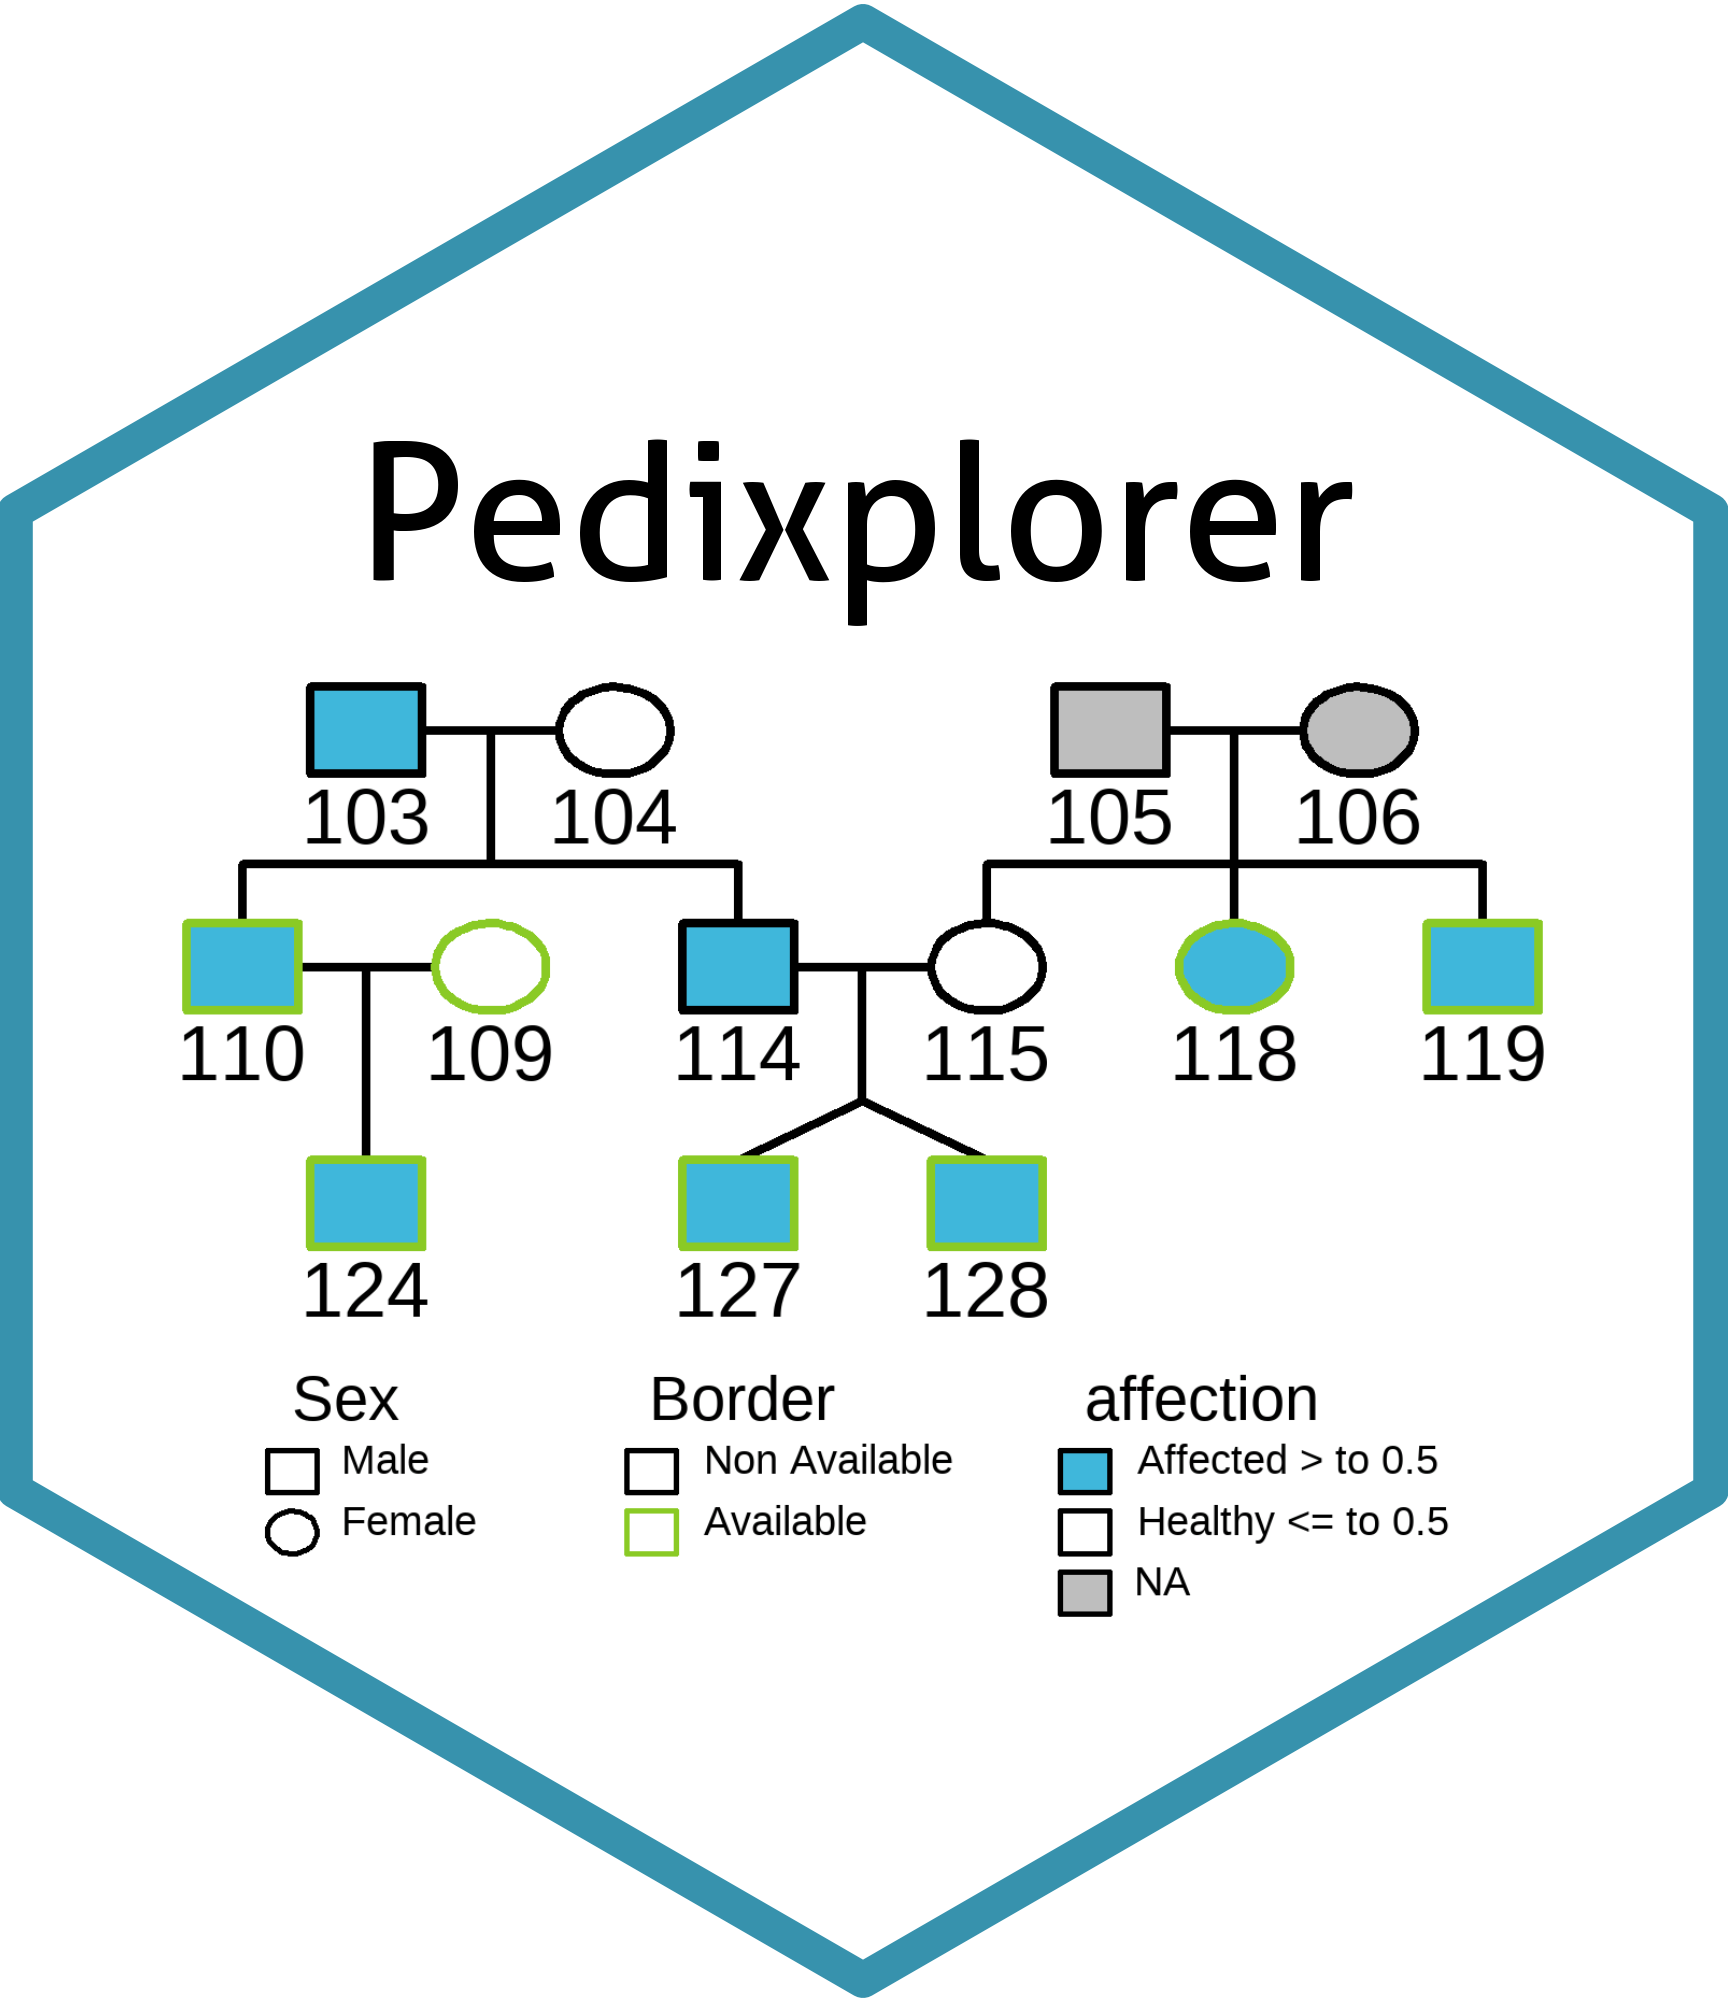
\includegraphics[width=0.4\linewidth]{../img/pedixplorer/icon_pedixplorer.png}}
            \href{https://nf-co.re/phaseimpute}{
\includegraphics[width=0.4\linewidth]{../img/phaseimpute/nf-core-phaseimpute_hexagonal_logo.png}}
        \end{minipage}
    } \\
    \href{https://www.bioconductor.org/packages/release/bioc/html/Pedixplorer.html}{Pedixplorer (v1.1.5)}
    & \textbf{Bioconductor} pedigree R package
    & \\
    \href{https://nf-co.re/phaseimpute}{Phaseimpute (v1.0.0)}
        & \textbf{nf-core} pipeline for phasing and imputation
        & \\
    & & \\
\end{tabularx}

\subsection{Articles}
\begingroup
\nocite{*}
\renewcommand{\section}[2]{}%
\printbibliography
\endgroup

% Section: Past Presentations
\section{Past Presentations}
    \subsection{Posters}
        \begin{itemize}
            \item \textit{Introducing nf-core/phaseimpute from idea to release} \newline
            Phd Symposium 2024 - Rennes and Nextflow Summit 2024 - Barcelona \\
            \item \textit{Imputation dans l'analyse génétique de la dysplasie de la hanche: une approche One Health chez le chien et l’Homme} \newline
            Assise de Génétiques 2024 - Paris and Atelier 281 Inserm 2024 - Bordeaux \\
            \item \textit{From Dog to Human: Searching the genetic bases of hip dysplasia} \newline
            IGDR Day 2023 - Rennes and ED SVS Scientific day 2024 - St-Malo \\
        \end{itemize}

    \subsection{Oral}
        \begin{itemize}
            \item \textit{Pedixplorer: A modern R BioConductor package for efficient kinship analysis to draw and request complex pedigrees} \newline
            EuroBioc 2024 – Oxford \\
            \item \textit{nf-core pipeline for genetic imputation: PhaseImpute} \newline
            Nextflow summit 2023 - Barcelona, PhD Symposium 2023 - Rennes, JOBIM 2024 - Toulouse \\
            \item \textit{La dysplasie de la Hanche du Chien à l’Homme} \newline
            MT180 Rennes and Brittany 2023 \\
        \end{itemize}

\end{document}
